\documentclass[tikz,border=2pt]{standalone}
% Estilo común de figuras y animaciones (mismos colores que la presentación)
% Compilar con XeLaTeX o LuaLaTeX (fuente TeX Gyre Heros); con pdfLaTeX usa Latin Modern Sans.
\usepackage{iftex}
\ifPDFTeX
  \usepackage[utf8]{inputenc}\usepackage[T1]{fontenc}\usepackage{lmodern}
  \renewcommand{\familydefault}{\sfdefault}
\else
  \usepackage{fontspec}\setmainfont{TeX Gyre Heros}\setsansfont{TeX Gyre Heros}
\fi
\usepackage{amssymb}
\usetikzlibrary{arrows.meta,positioning,calc,shapes.geometric,shadows,decorations.pathreplacing}
\definecolor{azul}{HTML}{1F3A5F}
\definecolor{acento}{HTML}{C0392B}
\definecolor{suave}{HTML}{EEF2F7}
\definecolor{gris}{HTML}{6B7280}
\definecolor{cOur}{HTML}{D62728}
\definecolor{cLib}{HTML}{1F77B4}
\definecolor{cWil}{HTML}{2CA02C}
\definecolor{cFol}{HTML}{FF7F0E}
\definecolor{cAnd}{HTML}{9467BD}
\definecolor{amarillo}{HTML}{F6C343}
\definecolor{verde}{HTML}{2E8B57}

% ---------- Iconos ----------
\providecommand{\iconscale}{1}
% \robot{pos}{color}{nombre}
\newcommand{\robot}[3]{%
  \begin{scope}[shift={#1}, scale=\iconscale, transform shape]
    \draw[#2, line width=0.8pt] (0,0.62) -- (0,0.78); \fill[#2] (0,0.8) circle (0.05);
    \draw[fill=#2!15, draw=#2, line width=0.8pt, rounded corners=2pt] (-0.3,0.25) rectangle (0.3,0.62);
    \fill[#2] (-0.13,0.45) circle (0.05); \fill[#2] (0.13,0.45) circle (0.05);
    \draw[#2, line width=0.6pt] (-0.1,0.33) -- (0.1,0.33);
    \draw[fill=#2!25, draw=#2, line width=0.8pt, rounded corners=2pt] (-0.24,-0.2) rectangle (0.24,0.22);
    \node[font=\tiny\bfseries, #2!70!black] at (0,-0.33) {#3};
  \end{scope}}
% \persona{pos}{color}{nombre}
\newcommand{\persona}[3]{%
  \begin{scope}[shift={#1}, scale=\iconscale, transform shape]
    \draw[fill=#2!20, draw=#2, line width=0.8pt] (0,0.5) circle (0.17);
    \draw[fill=#2!35, draw=#2, line width=0.8pt] (-0.27,-0.2) .. controls (-0.27,0.25) and (0.27,0.25) .. (0.27,-0.2) -- cycle;
    \node[font=\tiny\bfseries, #2!70!black] at (0,-0.33) {#3};
  \end{scope}}
% \libro{pos}{color}{texto}
\newcommand{\libro}[3]{%
  \begin{scope}[shift={#1}, scale=\iconscale, transform shape]
    \draw[fill=#2!25, draw=#2!80!black, line width=0.7pt, rounded corners=1pt] (-0.25,-0.32) rectangle (0.25,0.32);
    \fill[#2!80!black] (-0.25,-0.32) rectangle (-0.18,0.32);
    \node[font=\tiny\bfseries, align=center] at (0.035,0) {#3};
  \end{scope}}
% \letrero{pos}{texto principal}{tickets}
\newcommand{\letrero}[3]{%
  \begin{scope}[shift={#1}, scale=\iconscale, transform shape]
    \draw[fill=azul, draw=azul!60!black, rounded corners=2pt, line width=0.8pt] (-0.95,-0.32) rectangle (0.95,0.32);
    \foreach \i in {0,...,3} {\fill[cFol] (-0.85+\i*0.11,0.12) rectangle ++(0.08,0.12);}
    \foreach \i in {4,...,15} {\fill[amarillo!80] (-0.85+\i*0.11,0.12) rectangle ++(0.08,0.12);}
    \node[font=\tiny\bfseries, white] at (0,-0.12) {#2};
    \node[font=\tiny, cFol, anchor=south] at (-0.66,0.32) {#3};
  \end{scope}}
% \trituradora{pos}
\newcommand{\trituradora}[1]{%
  \begin{scope}[shift={#1}, scale=\iconscale, transform shape]
    \draw[fill=gris!25, draw=gris, line width=0.8pt] (-0.35,-0.25) rectangle (0.35,0.1);
    \draw[fill=gris!50, draw=gris] (-0.42,0.1) rectangle (0.42,0.2);
    \foreach \x in {-0.25,-0.12,0.01,0.14,0.27} {\draw[gris, line width=0.6pt] (\x,-0.25) -- (\x-0.03,-0.42);}
  \end{scope}}
% \ticket{pos}{color}
\newcommand{\ticket}[2]{%
  \begin{scope}[shift={#1}, scale=\iconscale, transform shape]
    \draw[fill=#2!30, draw=#2!80!black, line width=0.6pt] (-0.16,-0.09) -- (0.16,-0.09) -- (0.16,-0.03) arc (270:90:0.03) -- (0.16,0.09) -- (-0.16,0.09) -- (-0.16,0.03) arc (90:-90:0.03) -- cycle;
  \end{scope}}
% \contador{pos}{valor}{color}
\newcommand{\contador}[3]{%
  \node[scale=\iconscale, draw=#3, fill=white, line width=0.8pt, circle, inner sep=1.2pt, minimum size=0.42cm, font=\scriptsize\bfseries, text=#3] at #1 {#2};}

\begin{document}
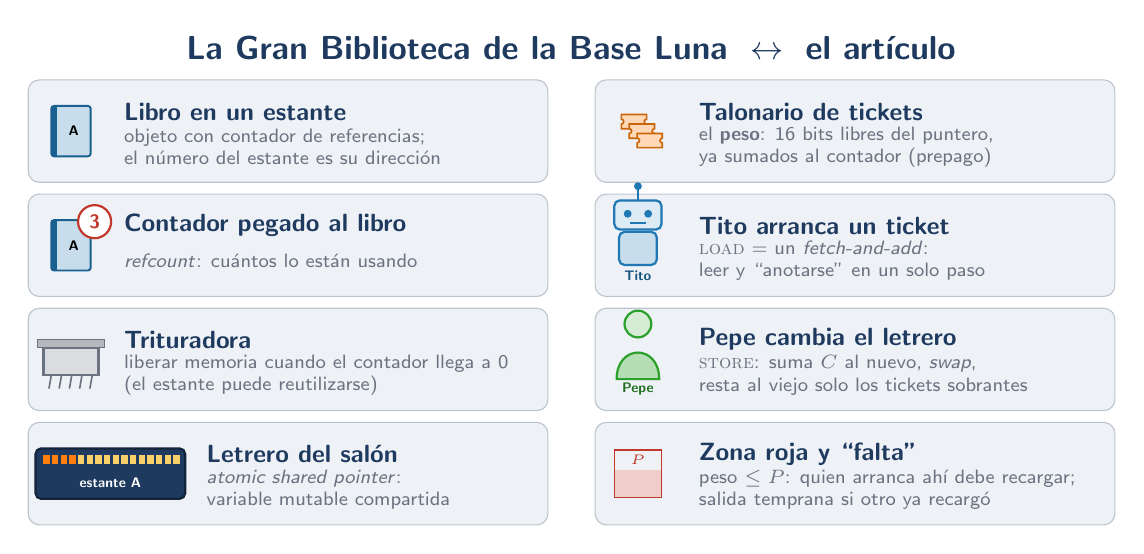
\begin{tikzpicture}[
    card/.style={draw=azul!30, fill=suave, rounded corners=4pt, minimum width=6.6cm, minimum height=1.3cm},
    hist/.style={font=\small\bfseries, text=azul, anchor=west},
    pap/.style={font=\scriptsize, text=gris, anchor=west, align=left},
    >=Stealth]
  % título
  \node[font=\large\bfseries, text=azul] at (6.9,4.15) {La Gran Biblioteca de la Base Luna \;$\leftrightarrow$\; el artículo};
  % columnas de tarjetas
  \foreach \col/\x in {0/0,1/7.2} {
    \foreach \row/\y in {0/3.1,1/1.65,2/0.2,3/-1.25} {
      \node[card, anchor=west] at (\x,\y) {};
    }
  }
  % --- columna izquierda
  \libro{(0.55,3.1)}{cLib}{A}
  \node[hist] at (1.1,3.35) {Libro en un estante};
  \node[pap]  at (1.1,2.9) {objeto con contador de referencias;\\ el número del estante es su dirección};

  \begin{scope}[shift={(0.55,1.65)}]
    \libro{(0,0)}{cLib}{A}\contador{(0.3,0.3)}{3}{acento}
  \end{scope}
  \node[hist] at (1.1,1.9) {Contador pegado al libro};
  \node[pap]  at (1.1,1.45) {\emph{refcount}: cuántos lo están usando};

  \trituradora{(0.55,0.25)}
  \node[hist] at (1.1,0.45) {Trituradora};
  \node[pap]  at (1.1,0.0) {liberar memoria cuando el contador llega a 0\\ (el estante puede reutilizarse)};

  \letrero{(1.05,-1.25)}{estante A}{}
  \node[hist] at (2.15,-1.0) {Letrero del salón};
  \node[pap]  at (2.15,-1.45) {\emph{atomic shared pointer}:\\ variable mutable compartida};

  % --- columna derecha
  \begin{scope}[shift={(7.75,3.1)}]
    \ticket{(-0.05,0.12)}{cFol}\ticket{(0.05,0)}{cFol}\ticket{(0.15,-0.12)}{cFol}
  \end{scope}
  \node[hist] at (8.4,3.35) {Talonario de tickets};
  \node[pap]  at (8.4,2.9) {el \textbf{peso}: 16 bits libres del puntero,\\ ya sumados al contador (prepago)};

  \robot{(7.75,1.6)}{cLib}{Tito}
  \node[hist] at (8.4,1.9) {Tito arranca un ticket};
  \node[pap]  at (8.4,1.45) {\textsc{load} = un \emph{fetch-and-add}:\\ leer y ``anotarse'' en un solo paso};

  \persona{(7.75,0.15)}{cWil}{Pepe}
  \node[hist] at (8.4,0.45) {Pepe cambia el letrero};
  \node[pap]  at (8.4,0.0) {\textsc{store}: suma $C$ al nuevo, \emph{swap},\\ resta al viejo solo los tickets sobrantes};

  \begin{scope}[shift={(7.75,-1.25)}]
    \fill[acento!25] (-0.3,-0.3) rectangle (0.3,0.05); \draw[acento] (-0.3,-0.3) rectangle (0.3,0.3);
    \node[font=\tiny\bfseries, acento] at (0,0.17) {$P$};
  \end{scope}
  \node[hist] at (8.4,-1.0) {Zona roja y ``falta''};
  \node[pap]  at (8.4,-1.45) {peso $\le P$: quien arranca ahí debe recargar;\\ salida temprana si otro ya recargó};
\end{tikzpicture}
\end{document}
